\section{Controls}
\ourgame{} will use standard first-person controls in order to allow players to navigate the 3D environment. These controls will require a keyboard and mouse. Mouse movement will be tied to the pitch and yaw of a perspective camera representing the player's view, and the \textbf{WASD} keys will control the character's movement within the world. Movement will be relative to the character's current facing, such that \textbf{W} will always cause the player to go forward, \textbf{S} will always cause them to go backward, and \textbf{A/D} will always strafe. Holding \textbf{Shift} will allow the player to run. Hitting \textbf{Space} will cause the player to jump.

When faced with a context-sensitive menu, such as those found in the UI described in Section~\ref{sec:UI_Gameplay}, the player may cycle through the options presented to them using the mouse's scrollwheel. The option that is currently in the foreground will be performed when the player presses the \textbf{Left Mouse Button}. When presented with an NPC's speech bubble, the player can press the \textbf{Left Mouse Button} in order to manually advance the conversation.

In order to navigate menus within \ourgame{}, the player will use mouse movement and clicks. Menus will contain text, buttons, and sliders. Text will be non-interactive. Buttons will be clickable and will give the user visual feedback based on the mouse's state in relation to the button. Sliders will be controlled by clicking the thumb and dragging it along the track or by clicking somewhere within the track, setting the thumb to that position.

To open the main menu from within the game, the user can press the \textbf{Escape} key. If the \textbf{Escape} key is pressed while the menu is open, the menu will close. The inventory menu can be opened and closed using the same method using the \textbf{Tab} key.

The yelling mechanic described in Section~\ref{sec:yelling_contest} will have two different control schemes based on whether the player is currently insulting or interrupting the opponent. When interrupting, the player must hit the \textbf{Space} key in order to attempt to interrupt. When insulting, the player must use \textbf{W} or \textbf{S} in order to choose which word/phrase is selected to complete the insult. 

The inventory system described in Section~\ref{sec:inventory} will be controlled using the mouse. While the inventory menu is open, a held item may be placed inside by clicking anywhere on the menu screen. This causes the item to be placed at the mouse's position. Similarly, items may be taken out of the inventory by clicking on them, as long as the player is not already holding an item.

\begin{figure}[H]
	\centering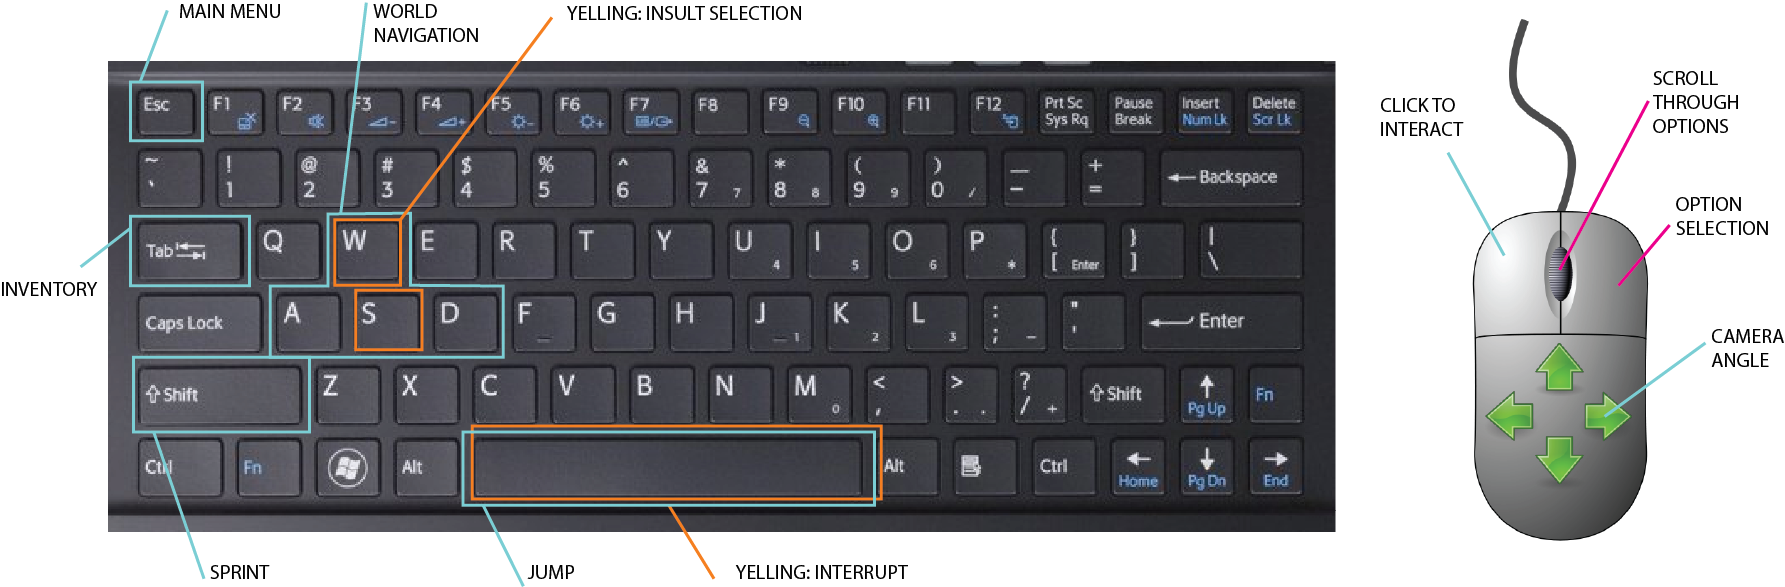
\includegraphics[width=.5\linewidth]{images/CONTROLS}
    \caption{All of the controls used for \ourgame{}}
    \label{fig:keyboard}
\end{figure}